\documentclass[aspectratio=169]{beamer}
\usetheme{Madrid}
\usepackage{physics}
\usepackage{bm}
\usepackage{pdfpages}
% Remove the automatic "Figure" label in captions for the presentation
\usepackage{caption}
\captionsetup[figure]{labelformat=empty}
\usepackage{xcolor} % ensure color package available
\definecolor{ff00ff}{HTML}{FF00FF} % define color #ff00ff
% Set background to black and all text to white
\definecolor{highlight}{HTML}{ffdb58} % new highlight color #ffdb58
\usecolortheme{default}
% set alerted text color (no bold)
%\setbeamercolor{alerted text}{bg=highlight}
% remove any bold setting: do NOT use \setbeamerfont{alerted text}{series=\bfseries}
% inline highlight: black text on colored background (with small padding)
\newcommand{\hlbg}[1]{\begingroup\setlength{\fboxsep}{3pt}\colorbox{highlight}{\strut\textbf{\textcolor{black}{#1}}}\endgroup}
% convenience macro for inline highlighted text (no bold)
\newcommand{\hl}[1]{{\color{highlight}#1}}

\definecolor{mywhite}{RGB}{255,255,255}
%\setbeamercolor{background canvas}{bg=white}
%\setbeamercolor{normal text}{fg=black}
% Define the blue color for footline
\definecolor{footlineblue}{HTML}{003DA5}

\setbeamercolor{frametitle}{bg=white, fg=footlineblue}
%\setbeamercolor{title}{bg=black, fg=mywhite}
%\setbeamercolor{section in toc}{fg=black}
%\setbeamercolor{subsection in toc}{fg=black}
%\setbeamercolor{item}{fg=black}
%\setbeamercolor{block title}{bg=black, fg=mywhite}
%\setbeamercolor{block body}{bg=black, fg=mywhite}

% Remove navigation symbols
\setbeamertemplate{navigation symbols}{}

% Remove the automatic section/subsection TOC at the top of each slide
\setbeamertemplate{headline}{}


% Show current slide number and total number of slides in footline

\definecolor{lightblue}{HTML}{D6E4F0}
% Show current slide number and total number of slides in footline
\begin{document}

\title{Chemfarm for collective quantum optics \\ Bonus: EM Green's functions} 
%\email{nikita.leppanen@weizmann.ac.il}
\author{Nikita Leppenen}
\date{February 2026}

\begin{frame}
    \titlepage
\end{frame}

\begin{frame}
    \frametitle{Vectorized 1D Greens function}
    \begin{figure}
        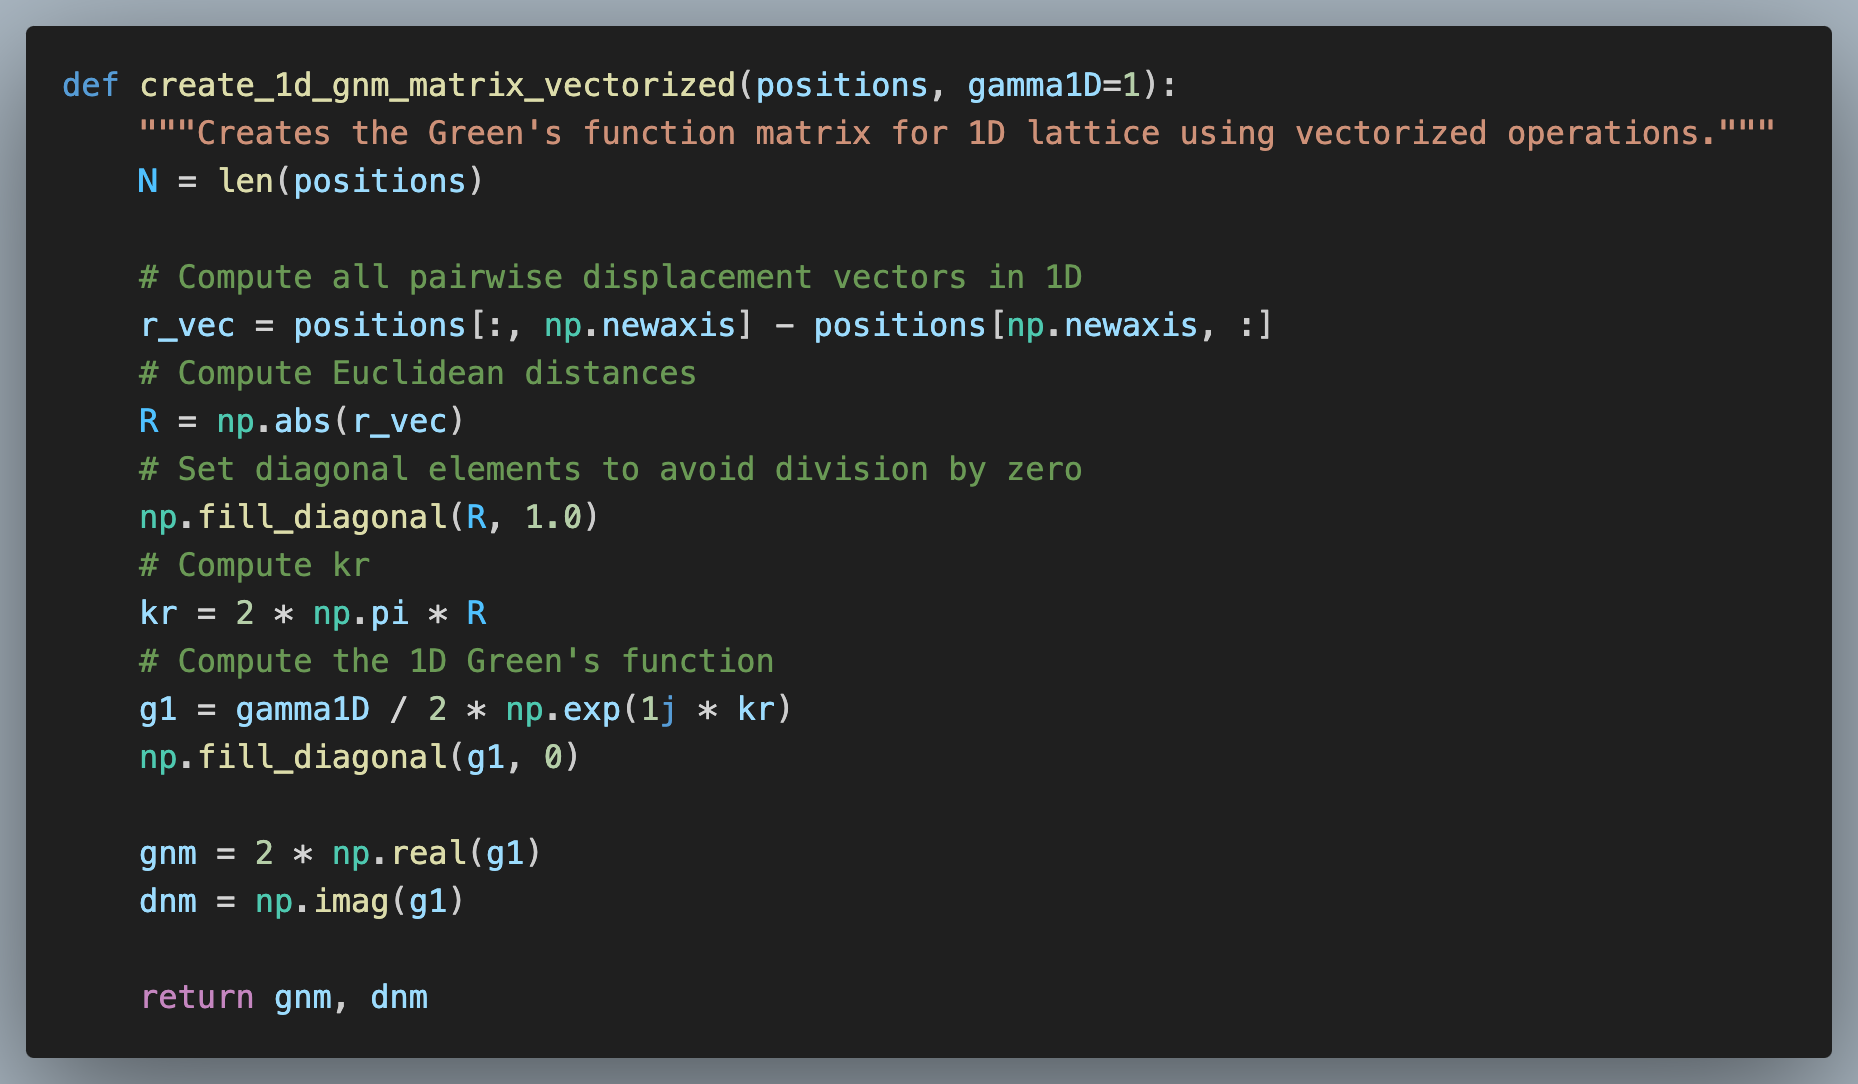
\includegraphics[width=0.8\textwidth]{img/1d_GF.png}
    \end{figure}
\end{frame}

\begin{frame}
    \frametitle{3D lattice with numpy}
    \begin{figure}
        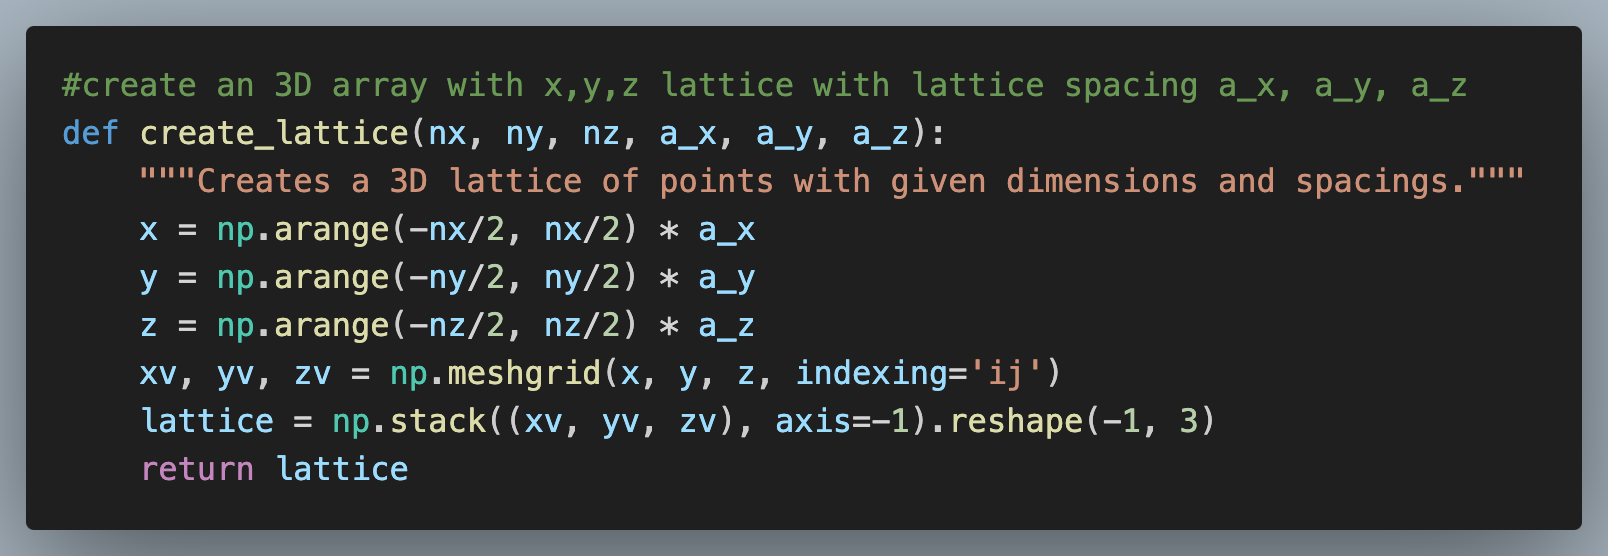
\includegraphics[width=0.8\textwidth]{img/3d_mesh.png}
    \end{figure}
\end{frame}

\begin{frame}
    \frametitle{3D Greens function with numpy}
    \begin{figure}
        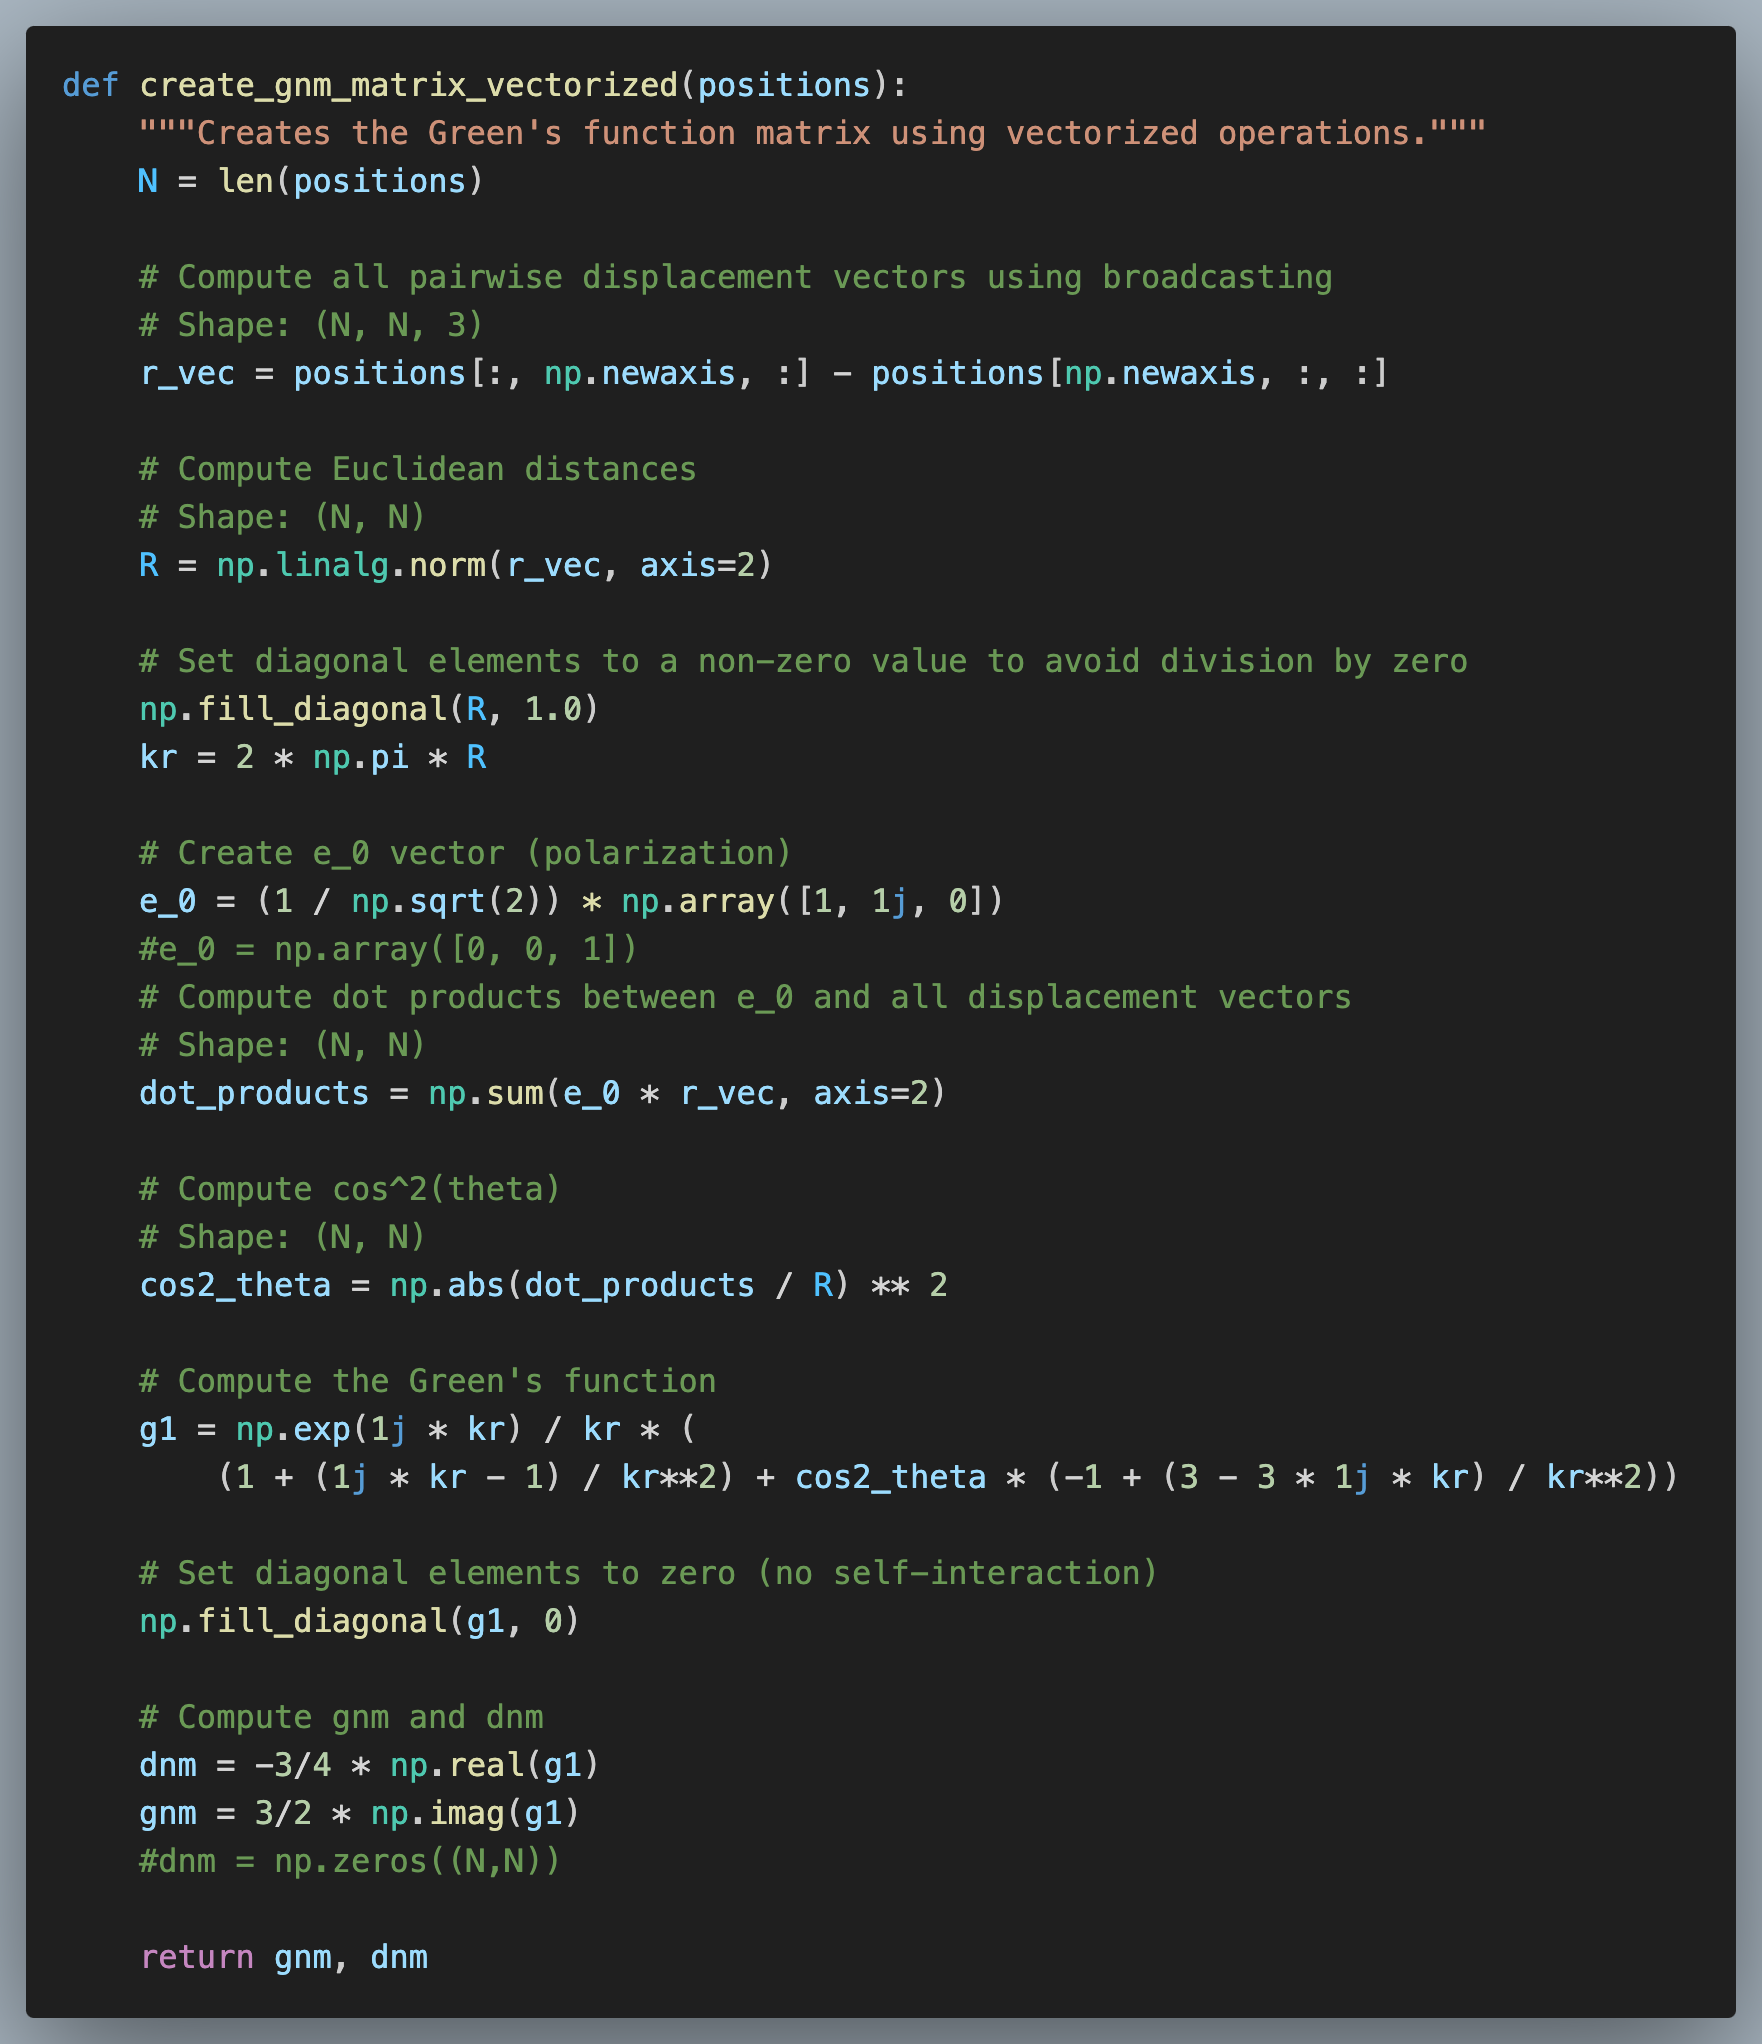
\includegraphics[width=0.8\textwidth]{img/3d_GF.png}
    \end{figure}
\end{frame}

\begin{frame}
    \vspace{-8cm}
    \hspace{1.5cm}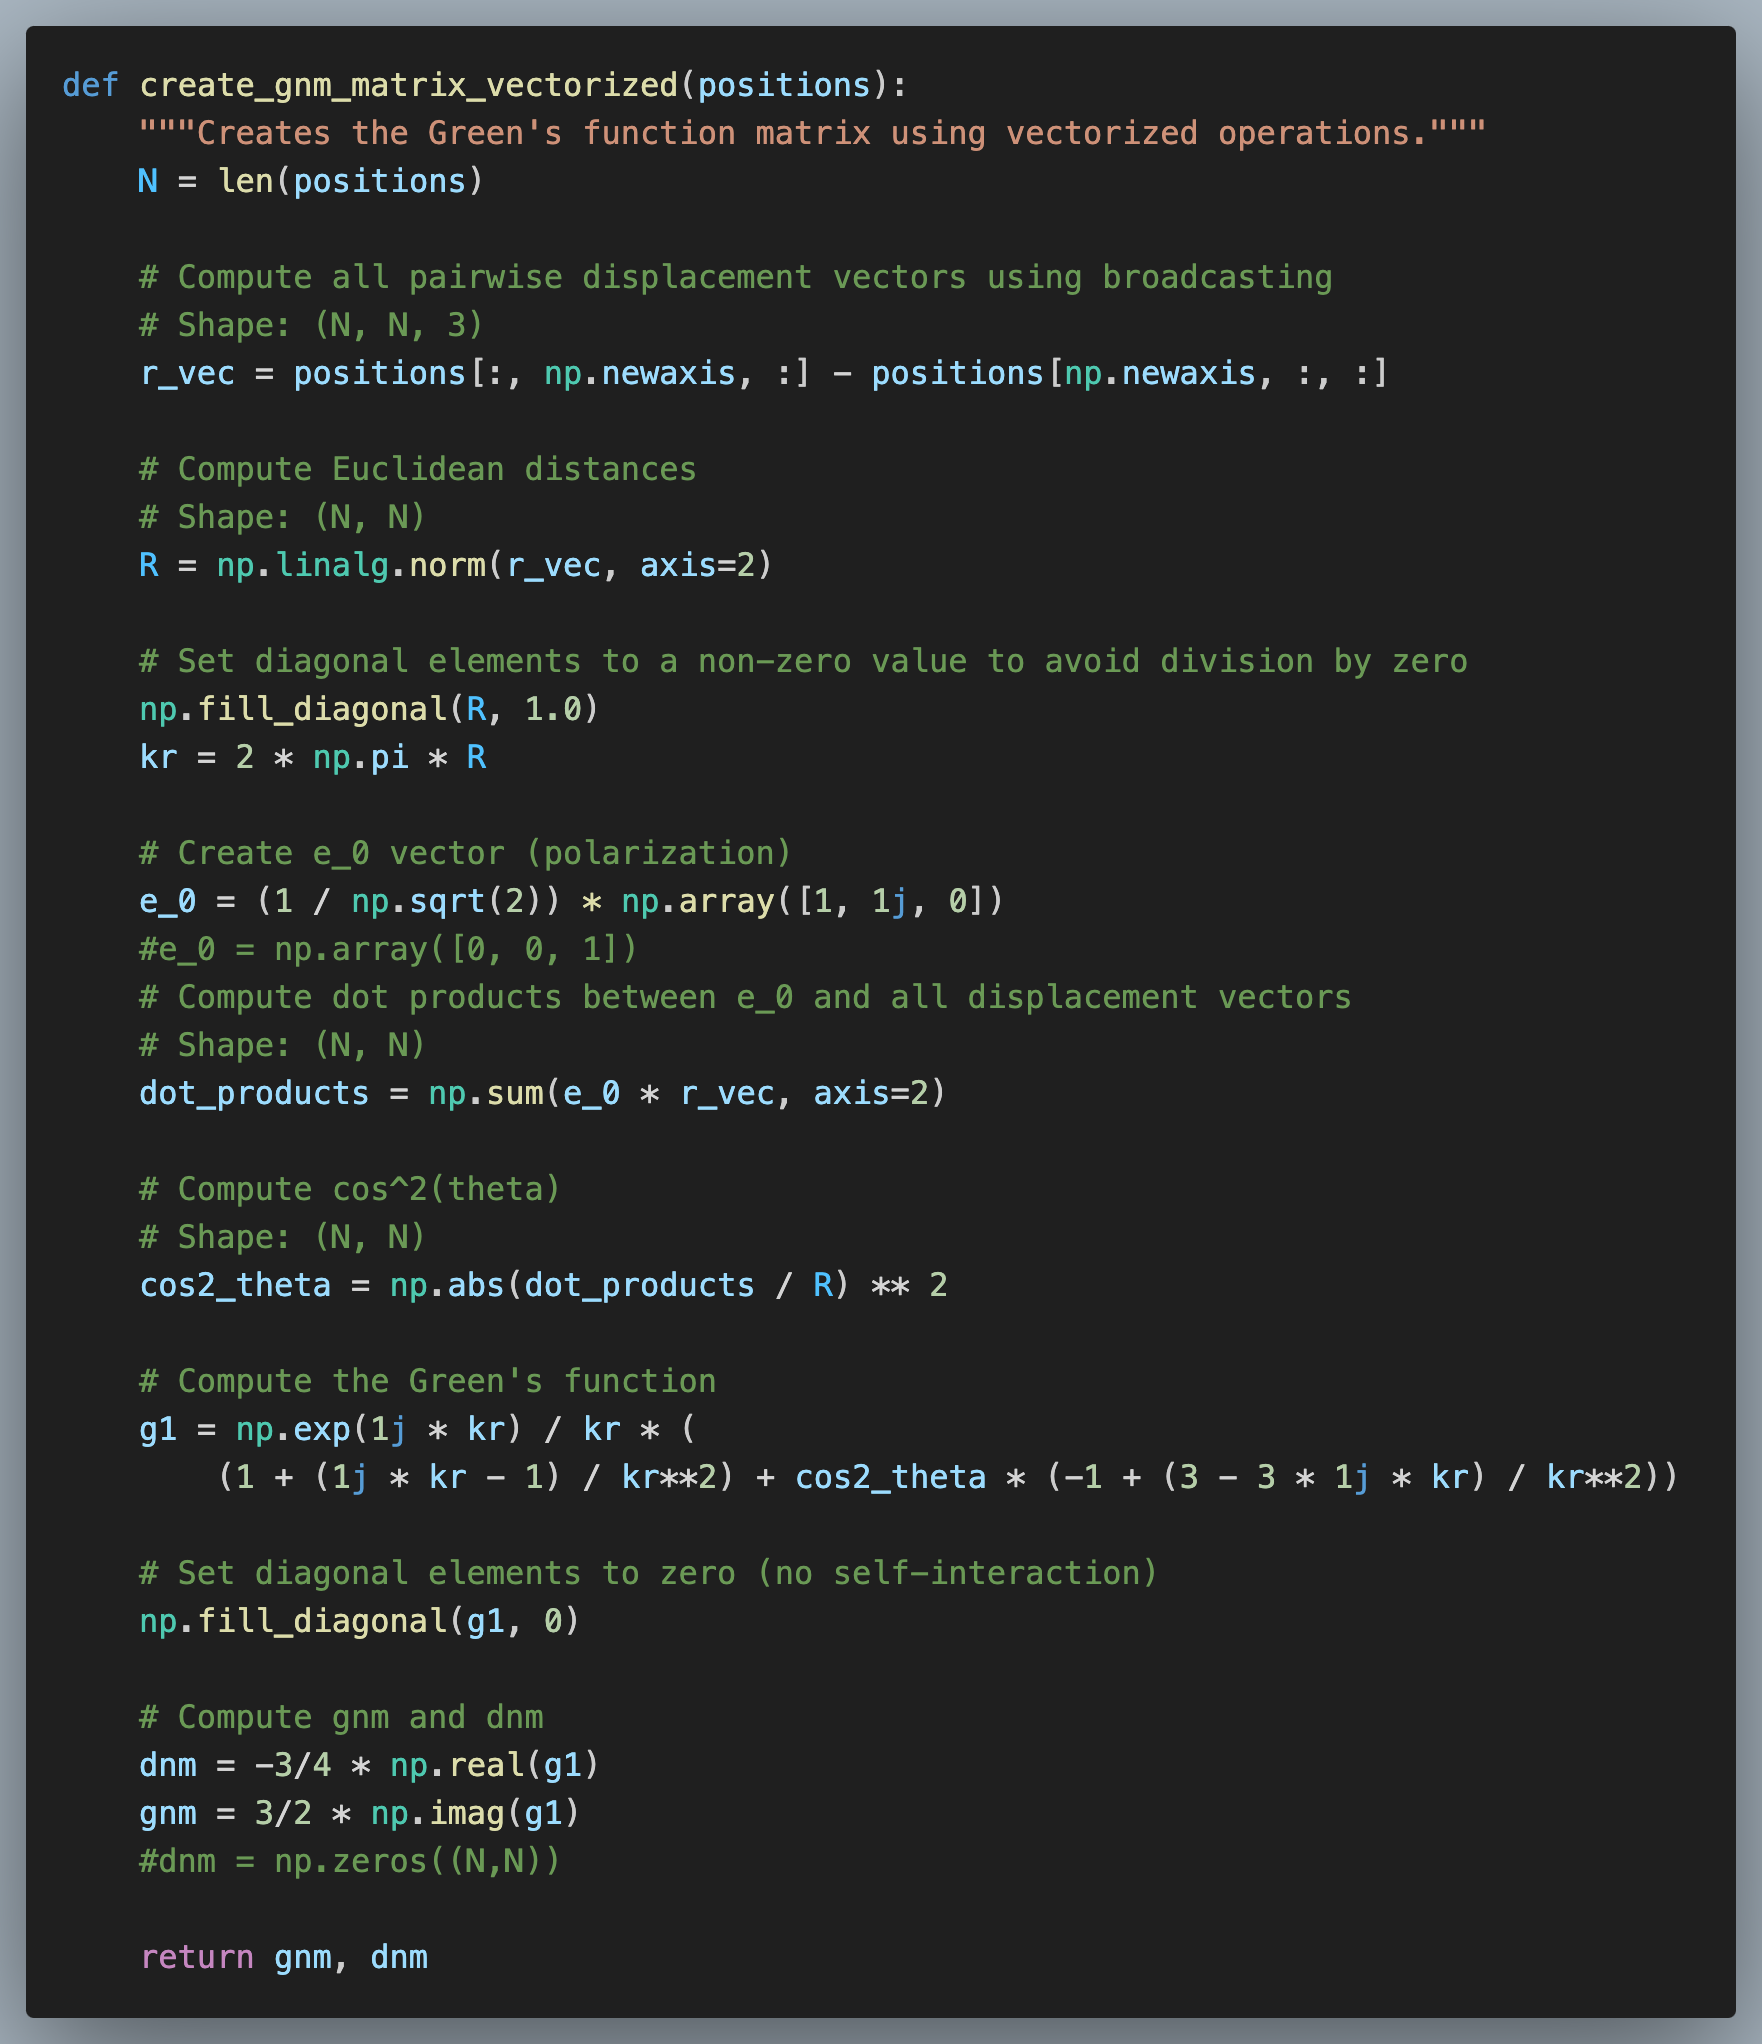
\includegraphics[width=0.8\textwidth]{img/3d_GF.png}
\end{frame}

\begin{frame}
    \frametitle{Example of 3D Greens function}

    \vspace{-0.2cm}
    \centerline{\scriptsize Code: 3DGF.py and $N_z = 1000$ on Chemfarm }

    \vspace{-0.2cm}
    \begin{figure}
        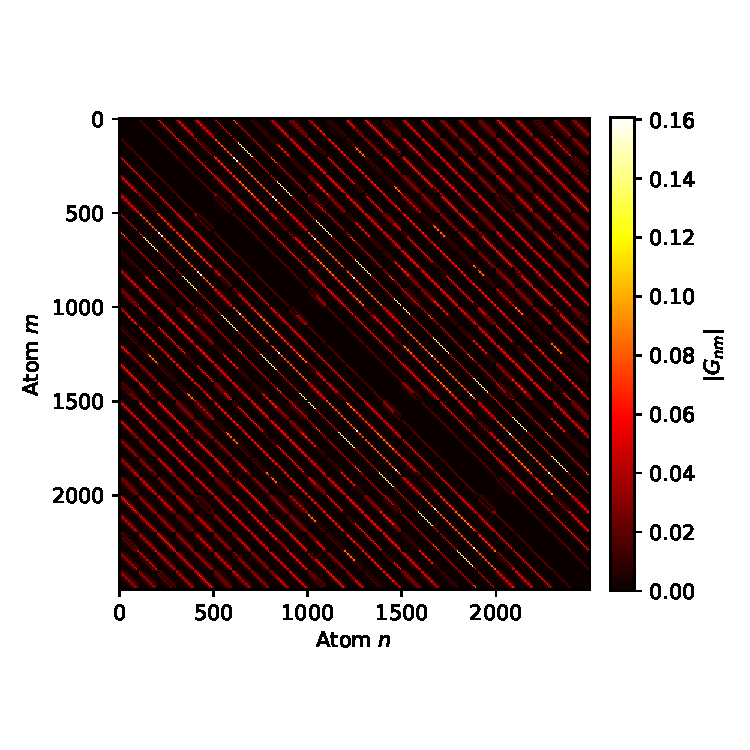
\includegraphics[width=0.45\textwidth]{img/gnm_matrix_5_5_100.pdf}
        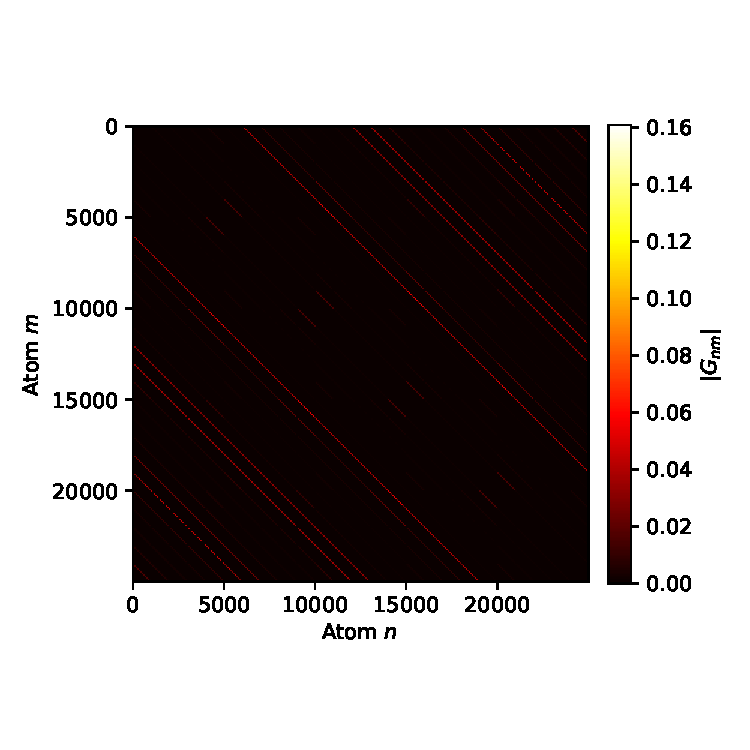
\includegraphics[width=0.45\textwidth]{img/gnm_matrix_5_5_1000.pdf}

        \vspace{-1cm}
        \caption{$|G_{nm}|$ for a 5x5 lattice in (xy) plane repeated 100 (left) and 1000 (right) times in z direction.\\ Spacing: $a_x = a_y = 0.5\lambda$ and $a_z = \lambda$. For $N_z = 1000$ -- sparse structure is seen -- {\color{red} could be studied!}} 
    \end{figure}
\end{frame}

\begin{frame}
    \frametitle{Experiments with sparce Green's function}

%Idea: do sparce full, then fill in translation invariant structure with 2D Green's function and then solve mean-field equations for the system. 



\end{frame}


\begin{frame}
    \frametitle{Appearence of 2D electrodynamics}
    Coherent $\Delta_{nm}$; incoherent $\gamma_{nm}$; $\frac{\gamma_{nm}}{2}+i\Delta_{nm} = -i \frac{3\gamma}{4}\bar{G}(\bm r_n - \bm r_m)$
    \begin{center}
    \textbf{$\lambda$ - spacing along $z$ $\Rightarrow$ system is (almost) translation invariant in $z$ direction.}

    3D Green's function (xyz) $\rightarrow$ 2D Green's function (xy - plane) between $z$ - chains of atoms.
    \end{center}

    1. Chain self interaction (without probe atom $m_z = n_z$):
    \begin{subequations}
\begin{multline*}
     \frac{\tilde{\gamma}_{n_\perp,n_\perp}}{2}+i\tilde{\Delta}_{n_\perp,n_\perp} = \sum_{m_z\neq n_z}\qty[\frac{\gamma_{n_\perp,n_z; n_\perp,m_z}}{2}+i\Delta_{n_\perp,n_z; n_\perp,m_z} ] = -i \frac{3\gamma}{4} \sum_{m_z\neq n_z} \bar{G}(\bm r_{n_\perp,n_z}-\bm r_{n_\perp,m_z})
\end{multline*}

    2. Interaction between different chains:
\begin{multline*}
     \frac{\tilde{\gamma}_{n_\perp,m_\perp}}{2}+i\tilde{\Delta}_{n_\perp,m_\perp} = \sum_{m_z} \qty[\frac{\gamma_{n_\perp,n_z; m_\perp,m_z}}{2}+i\Delta_{n_\perp,n_z; m_\perp,m_z} ] = -i \frac{3\gamma}{4} \sum_{m_z\neq n_z} \bar{G}(\bm r_{n_\perp,n_z}-\bm r_{m_\perp,m_z})
\end{multline*}
\end{subequations}
\end{frame}
\end{document}